
\section{Constrained Application Protocol}

An HTTP-inspired protocol designed for constrained devices and networks
used for RESTful access to resources. Default port is 5673 (coap) adn
5684(coaps). 

\begin{tabular}{lm{10cm}}
    Key features:&
\begin{itemize}
    \item Low overhead
    \item Easy to implement
    \item For Machine-2-Machine communication
    \item Simple mapping to HTTP for CoAP-HTTP proxies
\end{itemize}
\end{tabular}

CoAP messages provide reliable messaging over UDP and consist of a set of
method that resemble HTTP request methods and response code.
\begin{figure}[ht!]
    \centering
    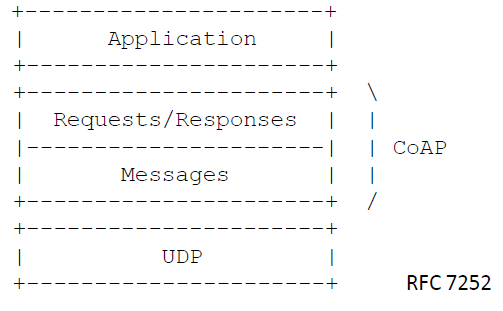
\includegraphics[width=0.5\linewidth]{img/coap-layer.png}
\end{figure}

\subsection{Message Format}
\begin{itemize}
    \item Messages are exchanged between UDP end-point
    \item they have the same format for request and response. 
    \item[$\rightarrow$]Header and options are in binary format.
\end{itemize}

\begin{figure}[ht!]
    \centering
    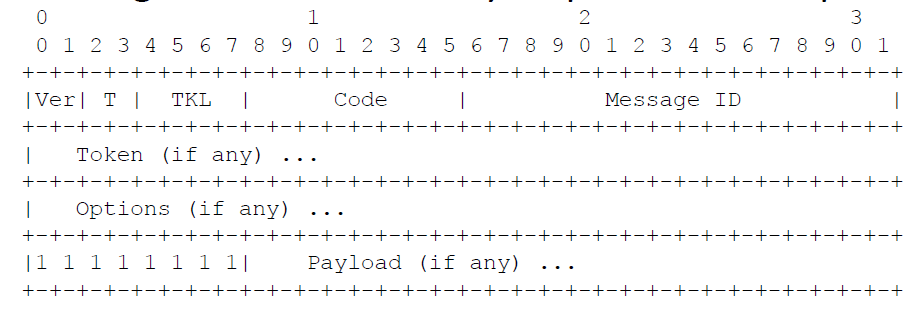
\includegraphics[width=0.5\linewidth]{img/coap-format.png}
\end{figure}

Message are compact $\Rightarrow$ avoid IP fragmentation and easy parsing.

\subsubsection{Fields}
\begin{description}
    \item[Ver:] Version number(01). Unknown versions are silently ignored.
    \item[Code:] \begin{tabular}{l}
            Method Code in request\\
            Response Code in responses
            \end{tabular}

        \begin{itemize}
            \item Method similar to HTTP: GET(0.01), POST(0.02), PUT(0.03), DELETE(0.04)
            \item Response codes similar to HTTP responses code: ok (2.05), not found
                (4.04),\ldots
            \item URI and additional options are stored in the options fields.
        \end{itemize}

    \item[Options:] Additional (0 or more) options, end marked by 1111111
        \begin{itemize}
            \item Options identified by their option code
            \item Option Code = Delta + previous option code
            \item Option length = length of option in bytes
            \item Delta is used to indicate presence of extension fields
        \end{itemize}
        
        \paragraph{URI} An URI such as
        \texttt{coap://example.com:5683/sensors/temp?x=1\&y=2} is not
        stored as one big string in a request but it is store as option.
        \begin{itemize}
            \item Host name in Uri-Host option (code 3)
            \item Port in Uri-Port option (code 7)
            \item Path segments in one or more Uri-Path options (without /)
            \item Query arguments in one or more Uri-Query (without \& and ?)
        \end{itemize}
        $\Rightarrow$ Simplifies parsing.

    \item[Token:] A 0 to 8 bytes value (length in TKL) generated by the
        client for concurrent request. Request for same
        source-destination should have unique token number.

        \begin{itemize}
            \item Response will use same number as the request
            \item Responses with unexpected token number are rejected
        \end{itemize}

        \paragraph{Security}
        CoAp connection can use \textbf{Datagram Transport Layer Security} which is like TLS but
        for UDP. If DTLS is not used, token should be long randomized token value to
        prevent response spoofing.

    \item[T:] Specifies the type of the message:
        \begin{itemize}
            \item Confirmable(0)
            \item Non-confirmable(1)
            \item Acknowlegment(2)
            \item Reset(3)
        \end{itemize}
\end{description}

\subsection{Transmission}
Depending on the type of the message, its treatment will be different.

\begin{itemize}
    \item \textbf{Transmission without Reliability}:
        Lightweight and useful for repeated operations, it applies to request or response
        of type \textcolor{red}{Non-confirmable}.
        \begin{itemize}
            \item Message might be sent multiple times by sender or network so each copy
                as a unique message ID to identify them.
            \item Message is ignored by recipient if unexpected or ill-formatted
                (unknown codes, wrong token value) $\to$ Recipient may send Reset 
                message with same message ID
        \end{itemize}

    \item \textbf{Transmission with Reliability}
        This applies to message of type \textcolor{red}{Confirmable}, Message ID
        is crucial but not only for de-duplication. Indeed, recipient must either
        reply with:
        \begin{itemize}
            \item Acknowledgement (with same message ID) or 
            \item Reset (with same msg ID) and ignore the message
        \end{itemize}

        Sender retransmits Confirmable message until ACK or Reset received 
        (or runs out of attempts).

        \paragraph{Retransmission} Exponential back-off

\begin{lstlisting}[frame=single]
    ACK_TIMEOUT = 2s
    ACK_RANDOM_FACTOR = 1.5
    MAX_RETRANSMIT = 4

    timeout := rand(ACK_TIMEOUT, ACK_TIMEOUT*ACK_RANDOM_FACTOR)
    retransmission-counter := 0

SENT: 
    send CON message
    wait until timeout or ACK or RESET
    if timeout and retransmission-counter < MAX_RETRANSMIT:
        timeout := timeout*2
        retransmission-counter++
        go to SENT
\end{lstlisting}
\end{itemize}

\subsection{Message Exchange}

\subsubsection{Synchronous Message Exchange}
\begin{minipage}{0.5\textwidth}
    \begin{figure}[H]
        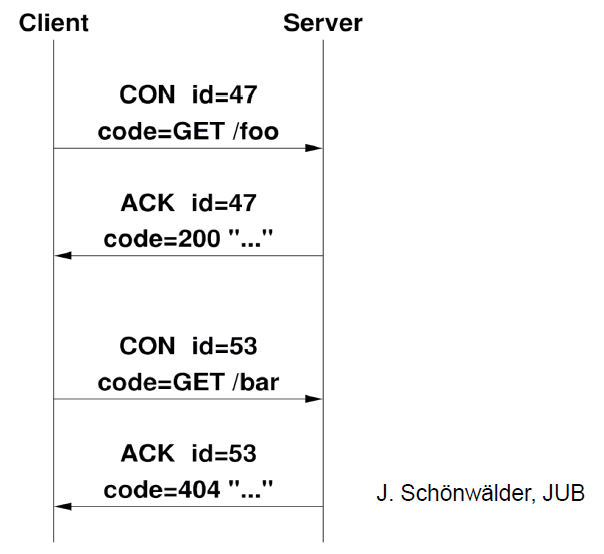
\includegraphics[width=0.5\linewidth]{img/syn-exchange.png}
    \end{figure}
\end{minipage} \hfill
\begin{minipage}{0.45\textwidth}
    \begin{itemize}
        \item Request sent as CON message
        \item Response sent as ACK message (piggybacking)
        \item Efficient
    \end{itemize}
\end{minipage}


\subsubsection{Asynchronous Message Exchange}
\begin{minipage}{0.5\textwidth}
    \begin{figure}[H]
        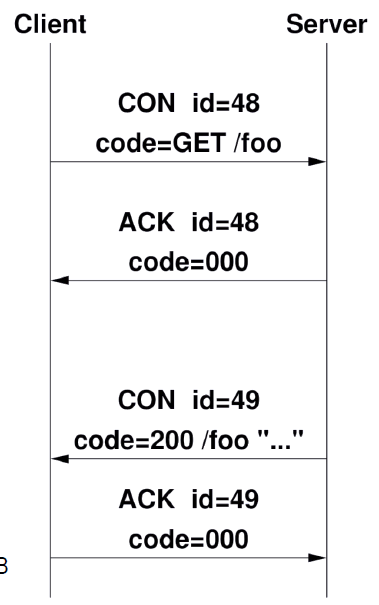
\includegraphics[width=0.5\linewidth]{img/asyn-exchange.png}
    \end{figure}
\end{minipage} \hfill
\begin{minipage}{0.45\textwidth}
    \begin{itemize}
        \item Request sent as CON message
        \item Recipient replies immediatel with empty ACK message (code 0.00)
        \item Recipient replies later with actual response in CON message
        \item More overhead than piggybacking
        \item Tokens for matching request <-> response
    \end{itemize}
\end{minipage}

\paragraph{Remarks}
\begin{itemize}
    \item CON and NON-CON messages can be mixed, ex: request as NON-CON and
        response as CON
    \item Empty CON (code 0.00) can be used as ping message, recipient replies with
        RESET message
    \item No definition of how long request should wait for response, CON-ACK 
        mechanism is only about reliable transmission
\end{itemize}

\subsection{CoAP Features}

\subsubsection{Multicasting and Discovery}
\begin{itemize}
    \item CoAP supports requests to IP multicast groups. Different behavior
        if request is multicast:
        \begin{itemize}
            \item Servers must not reply RESET to unwanted NON-CON messages 
                $\Rightarrow$ avoid too many error responses
            \item Servers should wait random time before responding request
                $\Rightarrow$ avoid congestion
        \end{itemize}
    \item Multicasting is useful for automatic service discovery in M2M scenarios.

    \item Servers should also support resource discovery:
        \begin{itemize}
            \item Client sends \texttt{GET ./well-known/core} to server
            \item Server returns list of resources
        \end{itemize}
\end{itemize}

\subsubsection{Caching}
CoAp uses a simple caching mode with an \textcolor{red}{age} option
indicating cache lifetime. 

$\Rightarrow$ This useful for proxies to cache information of sleeping nodes
or to reduce network traffic

\paragraph{Optional ETag}
\begin{enumerate}
    \item Server can put an ETag string in response
    \item Client sends ETag when re-requesting a cached resource
    \item Server can respond with 2.03 (valid) if resource has not
        changed
\end{enumerate}

ETag can be used in PUT-requests with \texttt{If-Match-Option}: Only write 
new value if I have latest one $\Rightarrow$ protection against accidental
concurrent overwrites

\subsubsection{Other Features}
\begin{itemize}
    \item Observing resources
    \item Block transfer (specify wanted bytes in request)
\end{itemize}

\subsection{Spoofing Attack}
CoAp runs over UDP, no handshake \& sequence number
\begin{itemize}
    \item Third party can spoof RESET message to disrupt connection
    \item CoAP endpoints can be used for amplication \& reflection 
        attacks against other targets.
\end{itemize}

Security (DTLS) and careful implementation (random token) can prevent attack
to some degree.

